\documentclass[a4paper,UTF8]{article}
\usepackage{ctex}
\usepackage[margin=1.25in]{geometry}
\usepackage{color}
\usepackage{graphicx}
\usepackage{amssymb}
\usepackage{amsmath}
\usepackage{amsthm}
\usepackage{enumerate}
\usepackage{bm}
\usepackage{hyperref}
\usepackage{epsfig}
\usepackage{color}
\usepackage{mdframed}
\usepackage{lipsum}
\usepackage{mathtools}
\usepackage{hyperref}
\usepackage{diagbox}
\usepackage{float}
\usepackage{caption}
\usepackage{algorithm}
\usepackage{algorithmicx}  
\usepackage{algpseudocode}
\usepackage{amsmath} 
\usepackage{graphicx}
\usepackage{subfigure}
\usepackage{url}
\newmdtheoremenv{thm-box}{myThm}
\newmdtheoremenv{prop-box}{Proposition}
\newmdtheoremenv{def-box}{定义}
\usepackage{listings}
\usepackage{xcolor}
\lstset{
	numbers=left, 
	numberstyle= \tiny, 
	keywordstyle= \color{ blue!70},
	commentstyle= \color{red!50!green!50!blue!50}, 
	frame=shadowbox, % 阴影效果
	rulesepcolor= \color{ red!20!green!20!blue!20} ,
	escapeinside=``, % 英文分号中可写入中文
	xleftmargin=2em,xrightmargin=2em, aboveskip=1em,
	framexleftmargin=2em
} 

\usepackage{booktabs}

\setlength{\evensidemargin}{.25in}
\setlength{\textwidth}{6in}
\setlength{\topmargin}{-0.5in}
\setlength{\topmargin}{-0.5in}

% \setlength{\textheight}{9.5in}
%%%%%%%%%%%%%%%%%%此处用于设置页眉页脚%%%%%%%%%%%%%%%%%%
\usepackage{fancyhdr}                                
\usepackage{lastpage}                                           
\usepackage{layout}                                             
\footskip = 10pt 
\pagestyle{fancy}                    % 设置页眉                 
\lhead{研一下学期}                    
\chead{论文阅读笔记}                                                
% \rhead{第\thepage/\pageref{LastPage}页} 
\rhead{Step7}                                                                                               
\cfoot{\thepage}                                                
\renewcommand{\headrulewidth}{1pt}  			%页眉线宽,设为0可以去页眉线
\setlength{\skip\footins}{0.5cm}    			%脚注与正文的距离           
\renewcommand{\footrulewidth}{0pt}  			%页脚线宽,设为0可以去页脚线

\makeatletter 									%设置双线页眉                                        
\def\headrule{{\if@fancyplain\let\headrulewidth\plainheadrulewidth\fi%
\hrule\@height 1.0pt \@width\headwidth\vskip1pt	%上面线为1pt粗  
\hrule\@height 0.5pt\@width\headwidth  			%下面0.5pt粗            
\vskip-2\headrulewidth\vskip-1pt}      			%两条线的距离1pt        
 \vspace{6mm}}     								%双线与下面正文之间的垂直间距              
\makeatother  

%%%%%%%%%%%%%%%%%%%%%%%%%%%%%%%%%%%%%%%%%%%%%%
\numberwithin{equation}{section}
%\usepackage[thmmarks, amsmath, thref]{ntheorem}
\newtheorem{theorem}{Theorem}
\newtheorem*{definition}{Definition}
\newtheorem*{solution}{Solution}
\newtheorem*{prove}{Proof}
\newcommand{\indep}{\rotatebox[origin=c]{90}{$\models$}}

\usepackage{multirow}

%--

%--
\begin{document}
\title{论文阅读笔记\\
Step7}
\author{MF1833063, 史鹏, spwannasing@gmail.com}
\maketitle

\newpage
\section{Answering while Summarizing:Multi-task Learning for Multi-hop QA with Evidence Extraction}
本文基于HotpotQA,提出了一个叫Query Focused Extractor (QFE)的模型,基于 extractive summarization模型,另外相比已有的模型,克服了预测evidence sentence之间相互独立的问题(通过使用RNN),以及引入了Multi-Task,
可以和任意的RC模型结合。亮点是即使QFE和一个简单的baseline RC模型结合起来,也能达到evidence extraction score上的SOTA效果。
\begin{figure}[H]
	\centering
	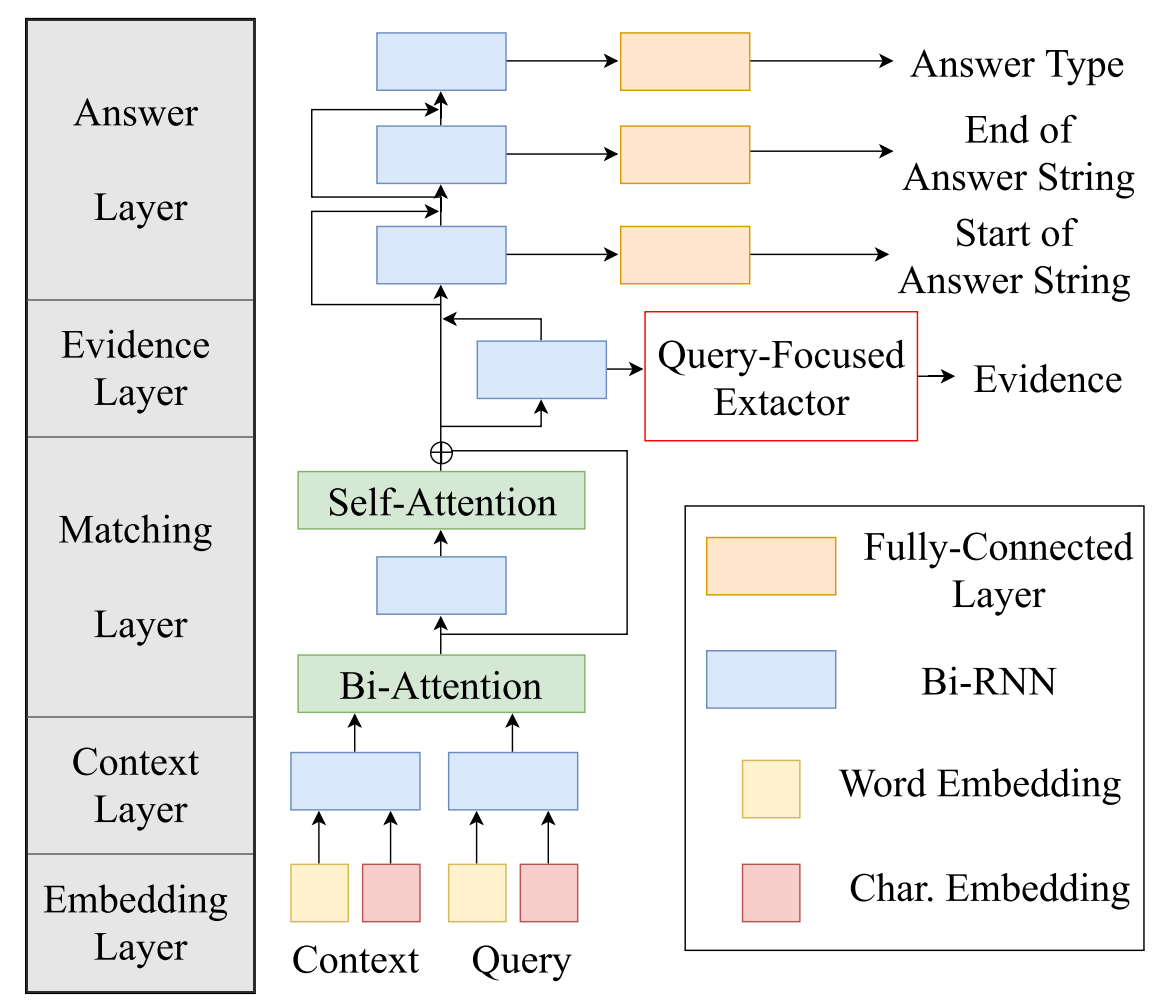
\includegraphics[width=0.6\textwidth]{1-1.png}
\end{figure}
\begin{figure}[H]
	\centering
	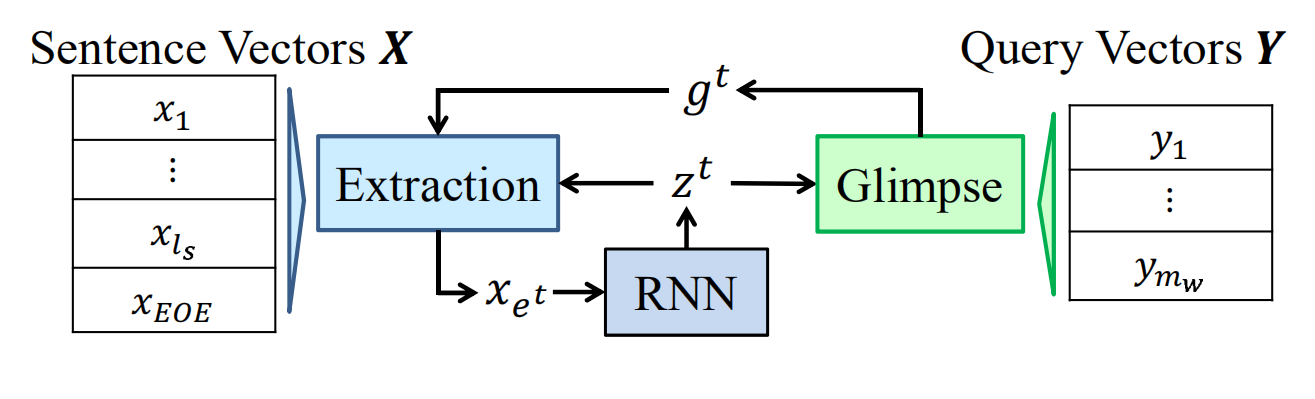
\includegraphics[width=0.6\textwidth]{1-2.png}
\end{figure}
\begin{equation}
	z^{t}=\mathrm{R} \mathrm{NN}\left(z^{t-1}, x_{e^{t}}\right) \in \mathbb{R}^{2 d_{c}}
	\end{equation}

	\begin{equation}
		\operatorname{Pr}\left(i ; E^{t-1}\right)=\operatorname{softmax}_{i}\left(u_{i}^{t}\right)
		\end{equation}
		\begin{equation}
		u_{i}^{t}=\left\{\begin{array}{ll}{v_{p}^{\top} \tanh \left(W_{p 1} x_{i}+W_{p 2} g^{t}+W_{p 3} z^{t}\right)} \\ {} & {\left(i \notin E^{t-1}\right)} \\ {-\infty} & {(\text { otherwise })}\end{array}\right.
		\end{equation}

	\begin{equation}
	\begin{aligned} g^{t} &=\sum_{j} \alpha_{j}^{t} W_{g 1} 1_{j} \in \mathbb{R}^{2 d_{c}} \\ \alpha^{t} &=\operatorname{softmax}\left(a^{t}\right) \in \mathbb{R}^{m_{w}} \\ a_{j}^{t} &=v_{g}^{\top} \tanh \left(W_{g 1} y_{j}+W_{g 2} z^{t}\right) \end{aligned}
	\end{equation}
	\begin{equation}
	\begin{aligned} L_{E}=-\sum_{t=1}^{|E|} & \log \left(\max _{i \in E \backslash E^{t-1}} \operatorname{Pr}\left(i ; E^{t-1}\right)\right) \\ &+\sum_{i} \min \left(c_{i}^{t}, \alpha_{i}^{t}\right) \end{aligned}
	\end{equation}
	\begin{equation}
		L=L_{A}+L_{E}
		\end{equation}

\newpage
\section{Do you know that Florence is packed with visitors?Evaluating state-of-the-art models of speaker commitment}
这篇论文展示出了带有语言学知识的模型的巨大潜力

对基于规则的和双向LSTM这两种最先进的说话人承诺模型进行了系统的评价

论文中的语言学分析给人启发,也展现出了系统的优势和劣势

当一个人,比如 Mary,问你「你知不知道佛罗伦萨全都是游客?」,我们会认为她相信佛罗伦萨全都是游客;但如果她问「你觉得佛罗伦萨游客多吗?」,我们就不会这样认为。推断说话人承诺(或者说事件真实度)是问答和信息提取任务中的关键部分。在这篇论文中,作者们探索了这样一个假说:语言学信息的缺乏会影响说话人承诺模型中的错误模式。他们的验证方式是在一个有挑战性的自然语言数据集上分析模型错误的语言学关联性。作者们在 CommitmentBank 这个由自然英语对话组成的数据集上评价了两个目前最好的说话人承诺模型。CommitmentBank 数据集已经经过了说话人承诺标注,方式是在 4 种取消蕴含的环境中向着时态嵌入动词(比如知道、认为)的补充内容进行标注。作者们发现,一个带有语言学知识的模型能展现比基于 LSTM 的模型更好的表现,这表明如果想要在这样的有挑战性的自然语言数据中捕捉这些信息的话,语言学知识是必不可少的。对语言学特征的逐项分析展现出了不对称的错误模式:虽然模型能在某些状况下得到好的表现(比如否定式),但它很难泛化到更丰富的自然语言的语言学结构中(比如条件句式),这表明还有很大提升的空间。

\begin{figure}[H]
	\centering
	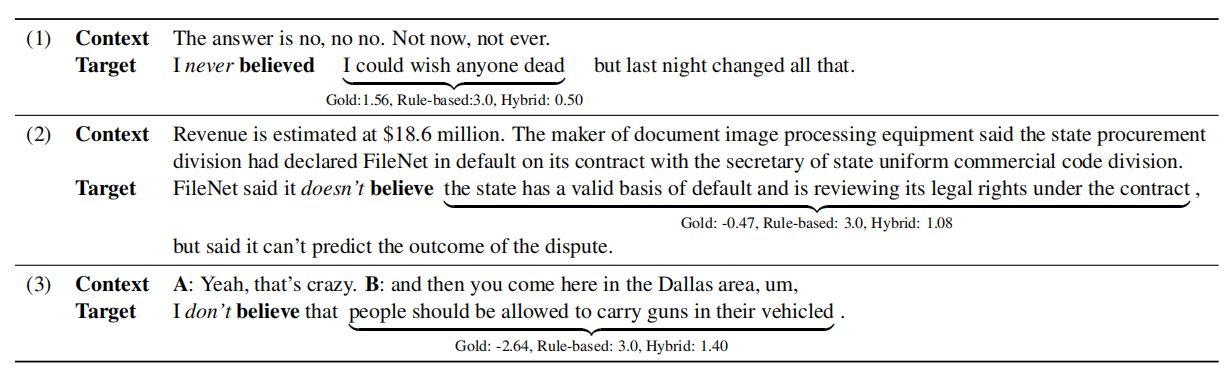
\includegraphics[width=\textwidth]{2-1.png}
\end{figure}

\newpage
\section{Emotion-Cause Pair Extraction:A New Task to Emotion Analysis in Texts}
情绪原因提取(Emotion cause extraction ,ECE)是一项旨在提取文本中某些情绪背后潜在原因的任务,近年来由于其广泛的应用而受到了很多关注。然而,它有两个缺点:1)情绪必须在ECE原因提取之前进行标注,这极大地限制了它在现实场景中的应用;2)先标注情绪然后提取原因的方式忽略了它们是相互指示的事实。

\begin{figure}[H]
	\centering
	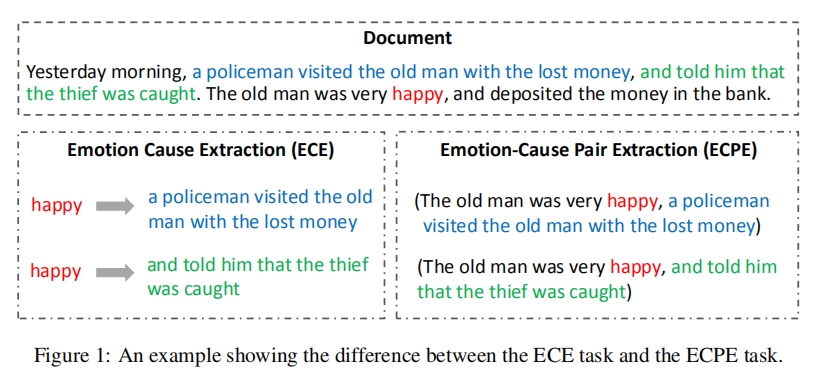
\includegraphics[width=\textwidth]{3-1.png}
\end{figure}
\begin{figure}[H]
	\centering
	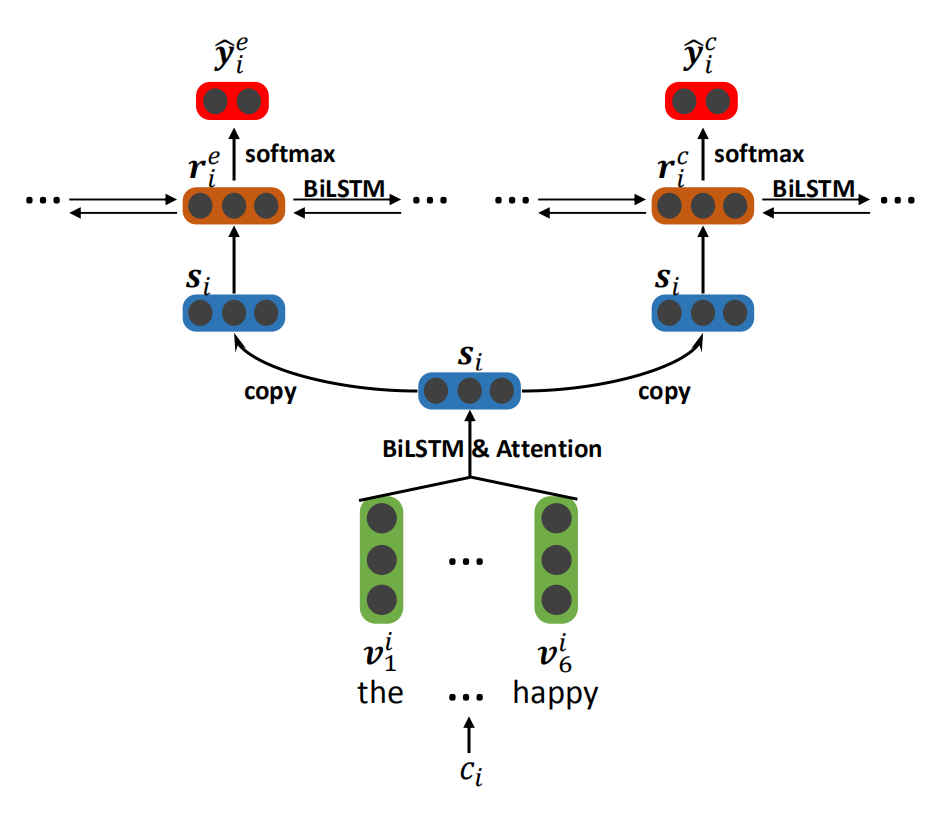
\includegraphics[width=0.8\textwidth]{3-2.png}
\end{figure}
\begin{figure}[H]
	\centering
	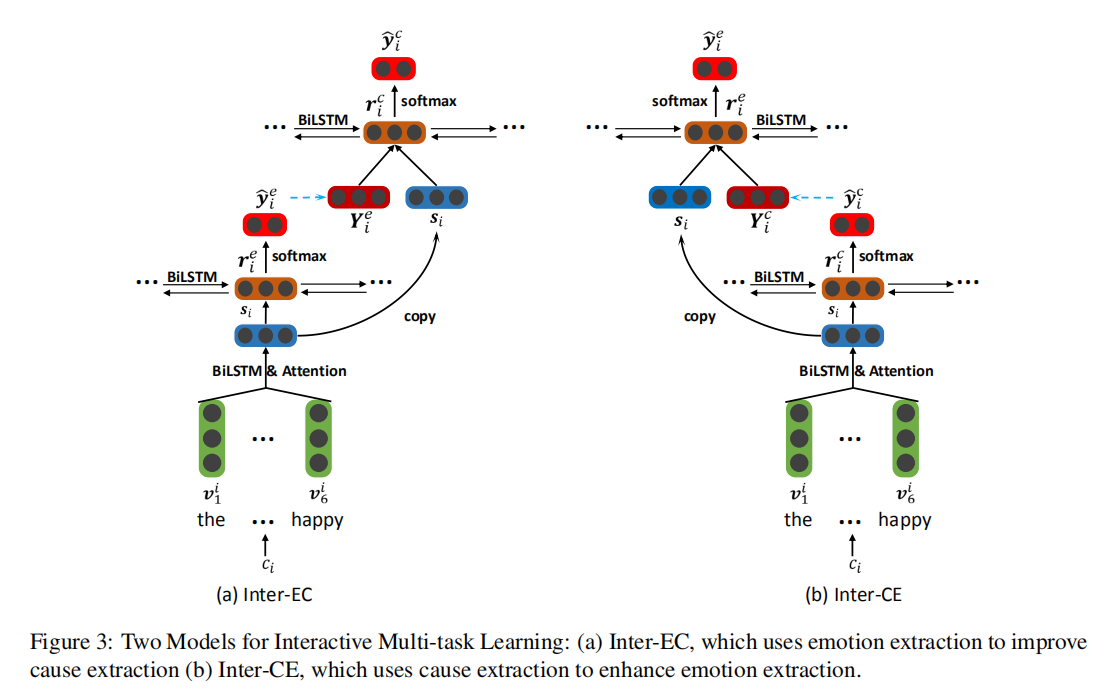
\includegraphics[width=\textwidth]{3-3.png}
\end{figure}

这篇文章的创新点就是提出了一个新的任务 emotion-cause pair extraction (ECPE),相较于传统的ECE不用依赖于事先的情感标注。
其次使用2-step的结构,第一步提取出E和C(有两种结构,一种E和C之间相互独立,另一种是有联系的),第二步进行筛选。

总体算法很简单,只使用了Bi-LSTM和attention结构,核心是提出一个新的Task。

\newpage
\section{Bridging the Gap between Training and Inference for Neural Machine Translation}
ACL19最佳论文

神经机器翻译(NMT)是以上下文为条件来预测下一个词,从而顺序地生成目标词。在训练时,它以ground truth词汇作为上下文进行预测;而在推理时,它必须从头开始生成整个序列。反馈上下文信息的这种差异会导致误差累积。此外,词级训练要求所生成的序列与ground truth序列之间严格匹配,这导致对不同的但合理的翻译的过度校正。在本文中,我们在模型训练中不仅从ground truth序列还从预测序列中来采样上下文,其中预测序列是用句子级最优来选择的。
\begin{figure}[H]
	\centering
	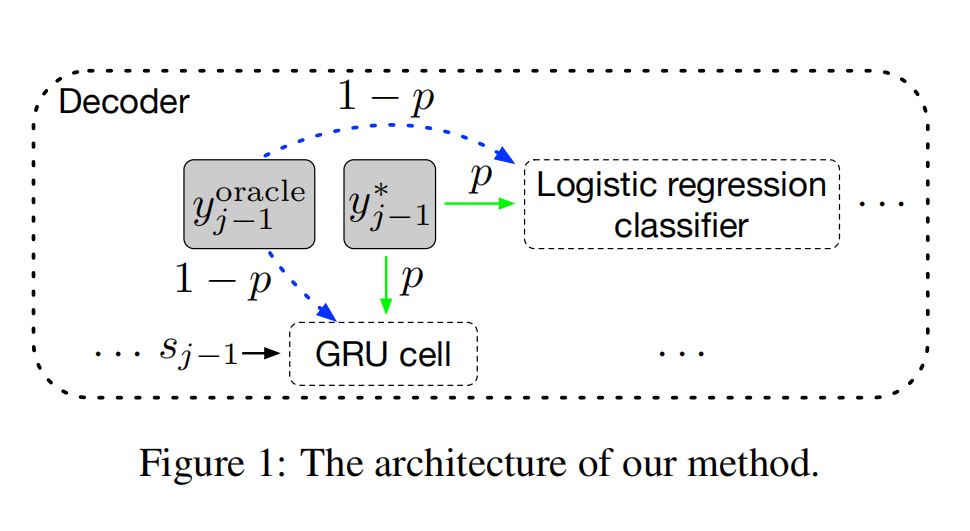
\includegraphics[width=0.6\textwidth]{4-1.png}
\end{figure}
\begin{figure}[H]
	\centering
	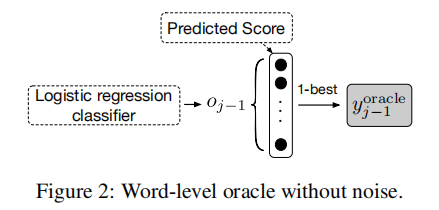
\includegraphics[width=0.6\textwidth]{4-2.png}
\end{figure}
\begin{figure}[H]
	\centering
	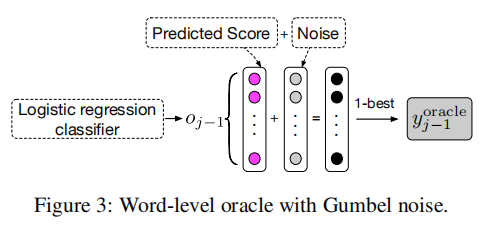
\includegraphics[width=0.6\textwidth]{4-3.png}
\end{figure}

\newpage
\section{Transferable Multi-Domain State Generator for Task-Oriented Dialogue Systems}
过度依赖领域本体和缺乏跨领域知识共享是对话状态跟踪的两个实际存在但研究较少的问题。现有方法通常在在推理过程中无法跟踪未知slot 值,且通常很难适应新领域。在本文中,我们提出了一个可转换对话状态生成器(Transferable Dialogue State Generator,TRADE)它使用复制机制从话语中生成对话状态,当预测在训练期间没有遇到的(domain,slot,value)三元组时可以促使知识转移。我们的模型由一个话语编码器、slot gate、状态生成器组成,它们跨域共享。实验结果表明,TRADE在人类对话数据集MultiWOZ的五个领域中实现了最先进的联合目标准确率48.62\%。
此外,我们通过模拟针对未见过的领域的zero-shot和few-shot对话状态跟踪,证明了其传输性能。在其中一个zero-shot域中TRADE实现了60.58\%的联合目标准确率,并且能够适应少数几个案例而不会忘记已经训练过的域。

\begin{figure}[H]
	\centering
	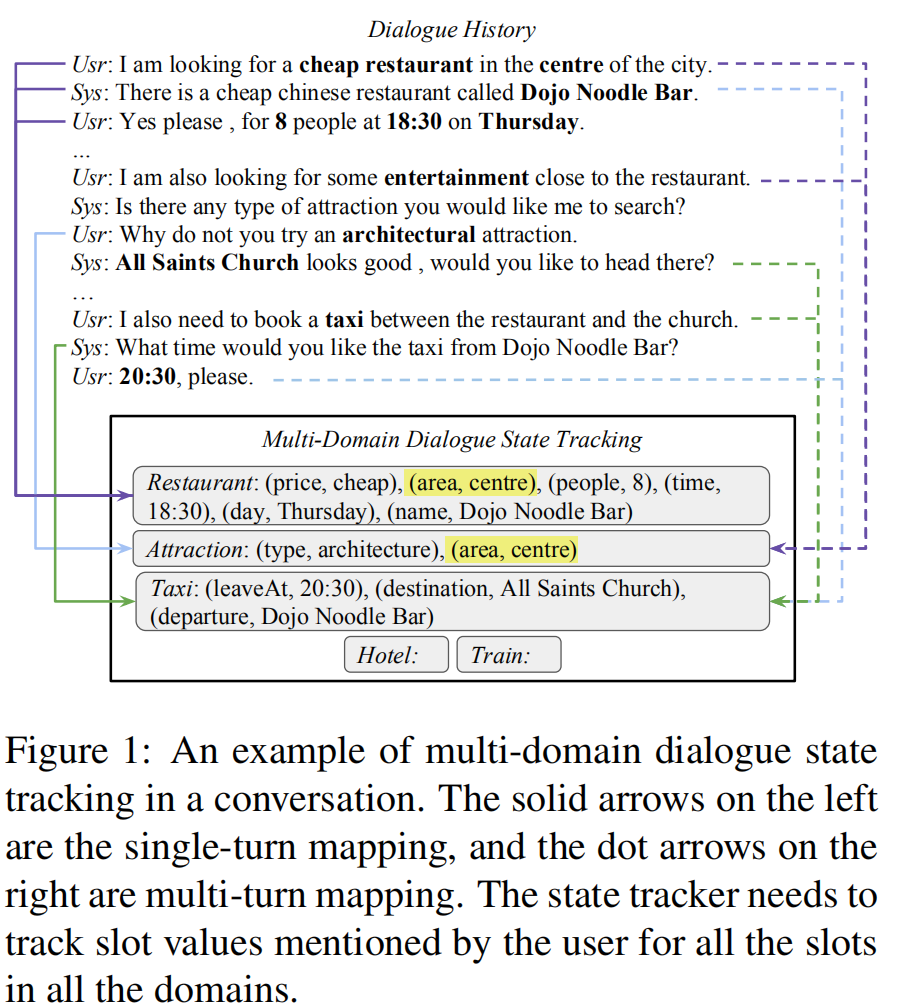
\includegraphics[width=0.6\textwidth]{5-1.png}
\end{figure}
\begin{equation}
\begin{aligned} P_{j k}^{\mathrm{vocab}} &=\operatorname{Softmax}\left(E \cdot\left(h_{j k}^{\mathrm{dec}}\right)^{\top}\right) \in \mathbb{R}^{|V|} \\ P_{j k}^{\mathrm{history}} &=\operatorname{Softmax}\left(H_{t} \cdot\left(h_{j k}^{\mathrm{dec}}\right)^{\top}\right) \in \mathbb{R}^{\left|X_{t}\right|} \end{aligned}
\end{equation}
\begin{equation}
\begin{aligned} P_{j k}^{\text { firal }} &=p_{j k}^{\text { gen }} \times P_{j k}^{\text { vocab }} \\ &+\left(1-p_{j k}^{\text { gen }}\right) \times P_{j k}^{\text { history }} \in \mathbb{R}^{|V|} \end{aligned}
\end{equation}
\begin{equation}
\begin{array}{c}{p_{j k}^{\mathrm{gen}}=\operatorname{Sigmoid}\left(W_{1} \cdot\left[h_{j k}^{\mathrm{dec}} ; w_{j k} ; c_{j k}\right]\right) \in \mathbb{R}^{1}} \\ {c_{j k}=P_{j k}^{\mathrm{history}} \cdot H_{t} \in \mathbb{R}^{d_{h d d}}}\end{array}
\end{equation}
\begin{figure}[H]
	\centering
	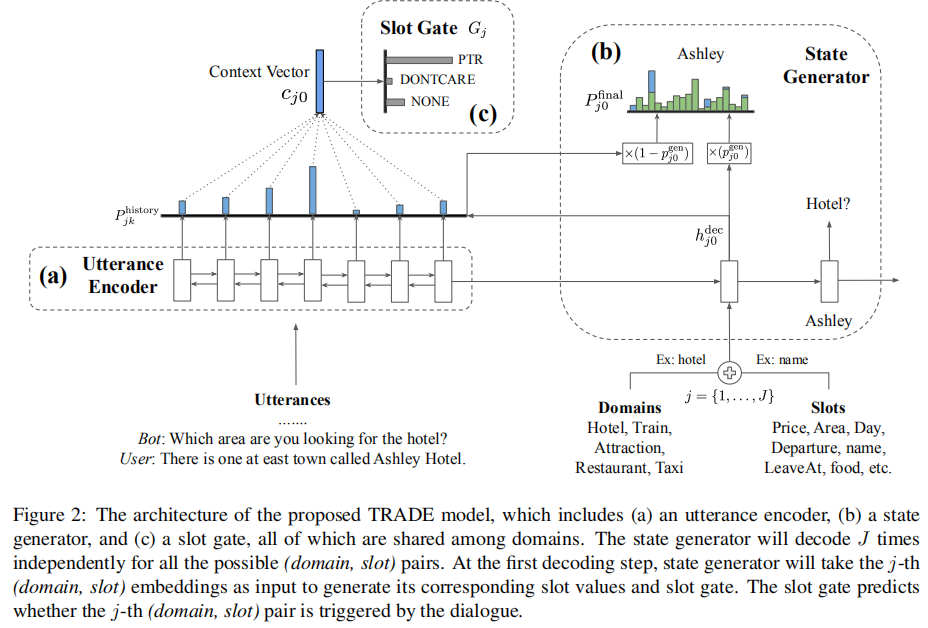
\includegraphics[width=\textwidth]{5-2.png}
\end{figure}


\newpage
\section{A Simple Theoretical Model of Importance for Summarization}

这篇文章讨论了自动文本摘要中长期存在的深层问题:

如何衡量摘要内容的适用性?

提出了「内容重要性」的三部分理论模型

提出了建设性的评估指标

文章中还与标准指标和人类判断进行了比较

摘要研究主要由经验方法驱动,手工精心调制的系统在在标准数据集上表现良好,但其中的信息重要性却处于隐含状态。 我们认为建立重要性(Importance)的理论模型会促进我们对任务的理解,并有助于进一步改进摘要系统。为此,我们提出了几个简单但严格定义的概念:冗余(Redundancy),相关性(Relevance)和信息性(Informativeness)。这些概念之前只是直观地用于摘要,而重要性是这些概念统一的定量描述。此外,我们提供了建议变量的直观解释,并用实验证明了框架的潜力以知道后续工作。

\newpage
\section{We need to talk about standard splits}
语音和语言技术的标准做法是根据在一个测试集上的性能来对系统进行排名。然而很少有研究人员用统计的方法来测试性能之间的差异是否是由偶然原因造成的,且很少有人检查同一个数据集中分割出不同的训练-测试集时的系统排名的稳定性。我们使用了2000年至2018年间发布的九个词性标注器进行复现实验,这些标注器每个都声称在广泛使用的标准的分割方式上获得了最佳性能。然而当我们使用随机生成的训练-测试集分割时,根本无法可靠地重现某些排名。我们在此建议使用随机生成的分割来进行系统比较。

本文质疑了评估NLP模型时公认且广泛运用的方法;

本文提出了几种关于数据集的标准拆分方法;

本文使用POS标记说明了问题;

本文建议系统排名应当基于使用随机分组的重复评估方法


\newpage
\section{Zero-Shot Entity Linking by Reading Entity Descriptions}
提出了zero-shot实体链接任务,其中mentions必须链接到没有域内标记数据的未曾见过的实体。这样做的目的是实现向高度专业化的领域的鲁棒迁移,也因此我们不会假设有元数据或别名表。在这种设置中,实体仅通过文本描述进行标记,并且模型必须严格依赖语言理解来解析新实体。首先,我们表明对大型未标记数据进行预训练的阅读理解模型可用于推广到未曾见过的实体。其次,我们提出了一种简单有效的自适应预训练策略,我们将其称为域自适应预训练(domain-adaptive pre-training ,DAP),DAP可以解决与在新域中链接未见实体的域迁移问题。我们在为此任务构建的新数据集上进行的实验,显示了DAP在强预训练基线(包括BERT)上有所改进。

本文提出了一种新颖的词义消歧系统,专门用于提高稀少的和未见过的词上的表现;

本文提出的感知选择任务被视为连续任务,并且使用了资源的组合;

本文的结果富有洞察力,并且改善了现有水平。

\begin{figure}[H]
	\centering
	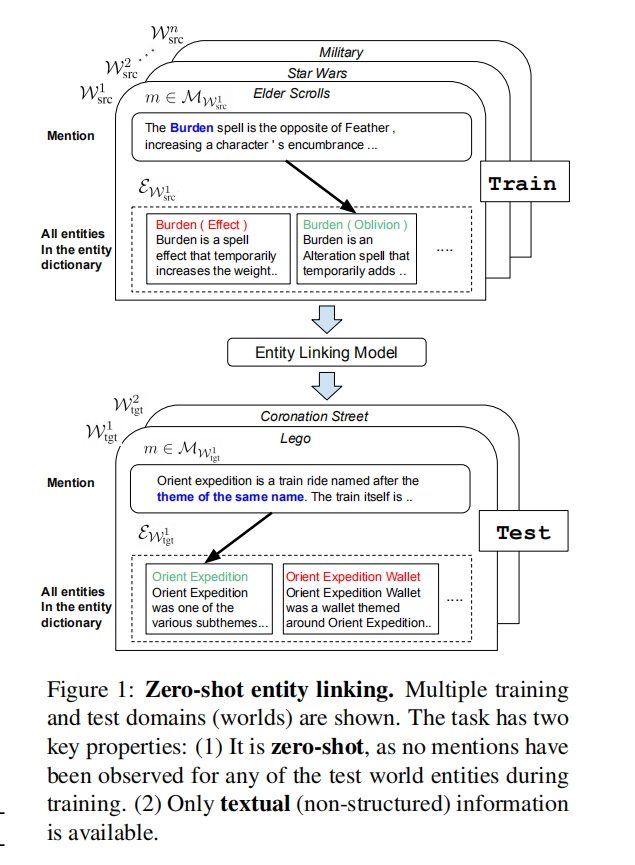
\includegraphics[width=0.6\textwidth]{8-1.png}
\end{figure}
\end{document}